\section{Filter}
Unter einem Filter (in der Elektrotechnik) versteht man eine Schaltung, bzw ein System das Frequenzen eines Signals selektiv dämpft.
Das Ziel hirbei ist es, dadurch das bestimmte Frequenzen durchgelassen werden während andere gedämpft werden, Rauschanteile
zu reduzieren und die Signalqualität zu verbessern. Er kann auch dazu genutzt werden, um SIgnale gezielt auf einen Frequenzbereich
zu begrenzen.
\\Es gibt vier primäre Filtertypen:
\begin{itemize}
    \item \textbf{Tiefpassfilter:} Niedrige Frequenzen werden durchgelassen, hohe Freuenzen werden gedämpft (Entfernung hoschfrquentes Rauschen)
    \item \textbf{Hochpassfilter:} Niedrige Frequenzen werden gedämpft, hohe Frequenzen werden durchgelassen (Entfernung DC-Anteile)
    \item \textbf{Bandpassfilter:} Lassen nur bestimmten Frequenzbereich durch (z.B. Kontrast zwischen Bildelemten erhöhen)
    \item \textbf{Bandsperrfilter:} Unterdrücken eine bestimmte Frequenz/Frequenzbereich (Bekannte Störungen bei bekannten Frequenzen entfernen)
\end{itemize}

In unserem Versuch wird ein Couoled-Line-Filter verwerwendet. Dieser ist Standardmäßig ein Bandpass.

\section{Prinzip von Coupled-Line-Filtern}
Ein Coupled Line Filter besteht aus zwei Parallelen Übertragungsleitungen (Transmission Lines), 
diese liegen so nahe beieinander, dass ihre elektromagnetischen Felder sich gegenseitig beeinflussen.
Diese elektromagnetische Kopplung hat Induktive sowie Kapazitive Anteile.
\\
Wird ein Hochfrequenzsignal über ein Coubled line Filter übertragen, hängt es stark
von der Frequenz des Signals ab, wie viel Leistung am Ausgang ankommt.
Da je nach Frequenz der Energieaustausch zwischen den Gekoppelten Leitungen effizienter oder weniger effizient ist.
Das kann man sich jedoch zu nutze machen, um gewünsche Frequenzen duch den Filter zu lassen und ungewünschte zu dämpfen bzw. sperren.

\section{Eigenschaften von Microstrip-Leitungen}
Microstip(Streifenleitung) gehören zu einer bestimmten Klasse der Wellenleiter.
Besonders in der Hochfrequenztechnik kommen sie zum Einsatz.
Um eine Microstrip-Leitung zu bauen, wird ein dünner Leitfähiger Streifen, wie Kupfer, auf einem Dielektrikum, wie FR4, aufgebracht.
\newpage
\section{Charakteristische Leitungslänge und Filterordnung}
Um die gewünschte Filtercharakteristik zu erreichen,
muss die Länge der Microstrip-Leitungen auf die Frequenz des Signals angepasst werden.
Typischerweise werden die Leitung als ein viertel der Wellelänge des Signals ausgelegt
$\lambda/4$. 
\\
Die Fitlerordung gibt an, wie viele parralele Übertragungsleitungen in einem Filter verbaut sind.
Werden z.B. drei gekoppelte Resonatorabschnitte verwenden spricht man von Filterordnung 3.
Durch höhere Filterordnungen kann die Steilheit des Amiltudengangs beim Übergang zwischen Durchlass- und Sperrberreich erhöht werden.
Was eine bessere selektierung der Frequenzen ermöglicht.


\section{Bedeutung der S-Parameter}
S-Parameter bzw. Streuparameter werden genutzt, um die HF-Eigenschaften eines
Netzwerks darzustellen. Sie werden benötigt, um zu verstehen, welche Anteile eines Signals
reflektiert, durchgelassen oder zwischen den Ports eines Netzwerks übertragen werden.
Sie werden komplex dargestellt, also mit Betrags- und Phasenkomponente.

Die Indexnummerierung folgt dem Energiefluss:

\begin{itemize}
    \item Verläuft die Energie von Port 1 zu Port 1, heißt der S-Parameter S11.
    \item Verläuft die Energie von Port 2 zu Port 1, heißt der S-Parameter S21.
\end{itemize}
Somit können an einem Zweitor folgende S-Parameter auftreten:
\begin{itemize}
    \item S11 ist der Eingangsreflexionsfaktor. Dieser Parameter gibt an, wie viel des Eingangssignals zurückreflektiert wird.
    \item S21 ist der Vorwärtstransmissionsfaktor. Dieser Parameter gibt die Effizienz der Signalübertragung vom Eingang zum Ausgang an.
    \item S12 ist der Rückwärtstransmissionsfaktor. Dieser Parameter gibt an, wie gut Port 1 von Signalen von Port 2 isoliert ist.
    \item S22 ist der Ausgangsreflexionsfaktor. Dieser Parameter gibt an, wie viel des Ausgangssignals zurückreflektiert wird.
\end{itemize}

\subsection{Smith-Diagramm}
Das Smith-Diagramm ermöglicht die grafische Darstellung der S-Parameter.
Dafür werden der Real- und Imaginärteil des Reflexionsfaktors in Abhängigkeit von der Frequenz
aufgetragen und ermöglichen dadurch eine einfachere Impedanzanpassung.
\begin{figure}[H]
    \centering
    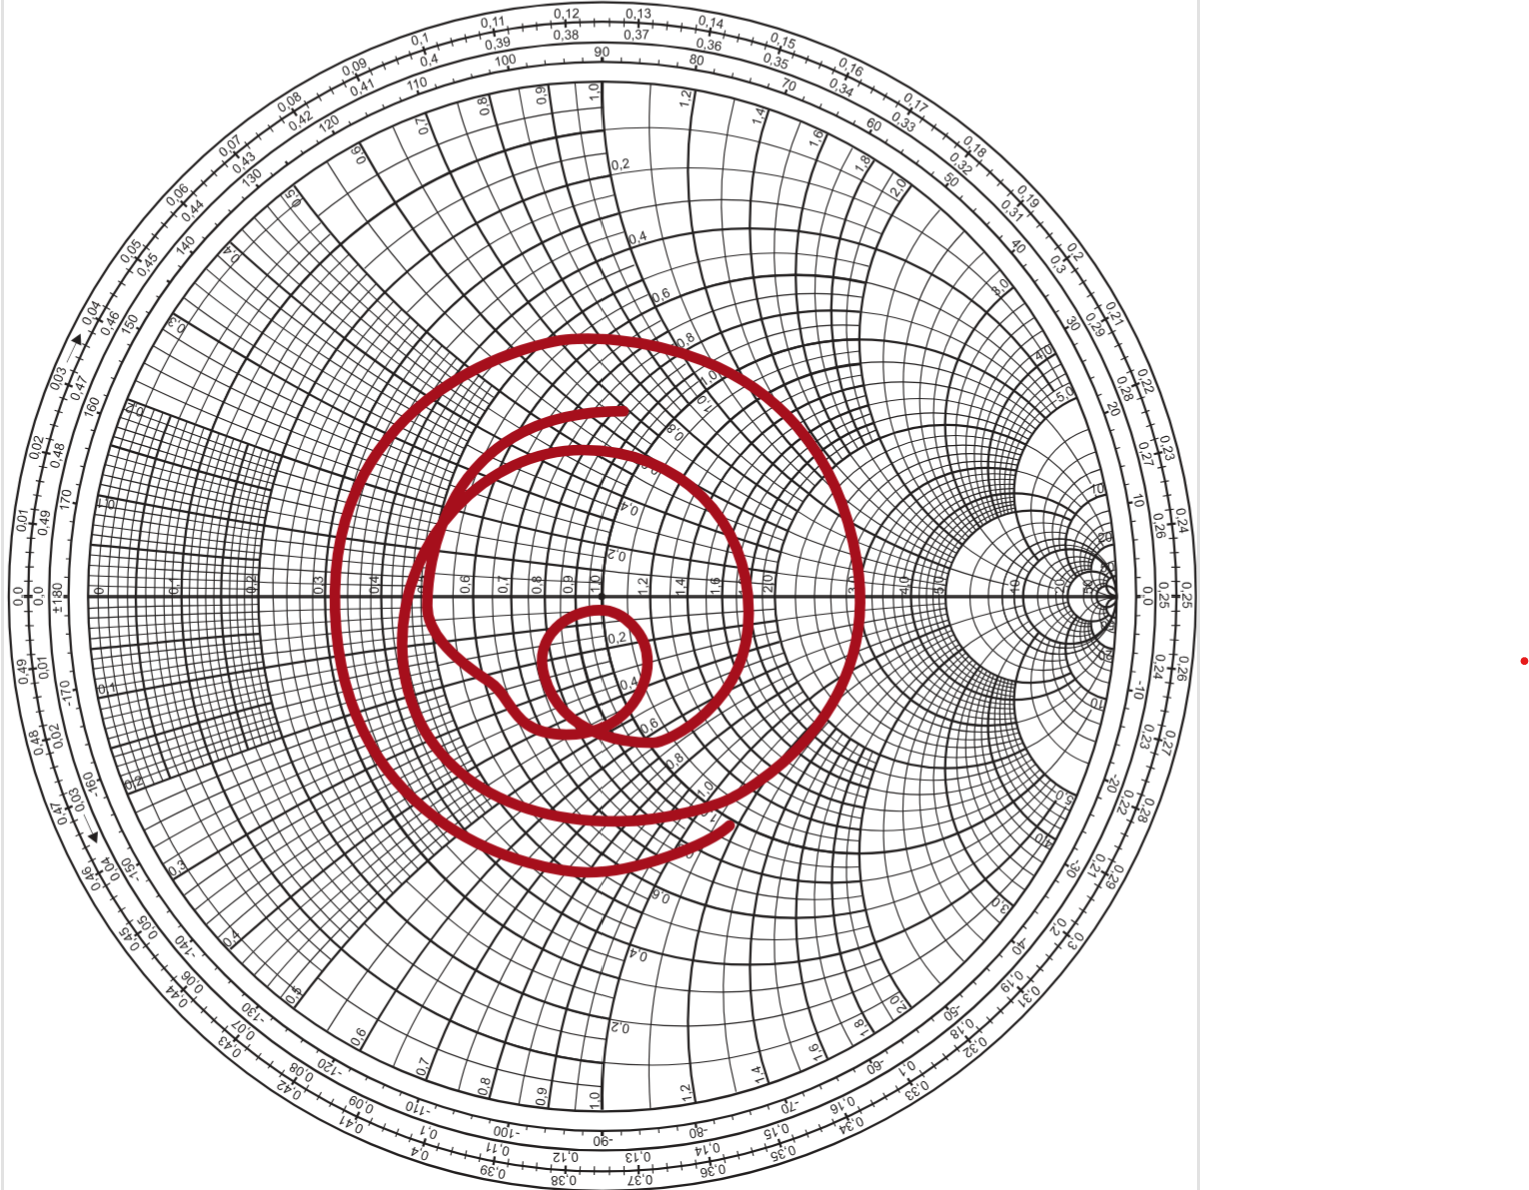
\includegraphics[width=0.4\textwidth]{Pictures/SmithDiagram.png}
    \caption{Smith-Diagramm Beispiel}
    \footnotesize{Quelle: \url{https://www.rohde-schwarz.com/de/produkte/messtechnik/essentials-test-equipment/spectrum-analyzers/s-parameter-verstehen_257831.html#gallery-13}}
\end{figure}

\clearpage